\section{Finanzen}

\begin{figure}[H]
\centering
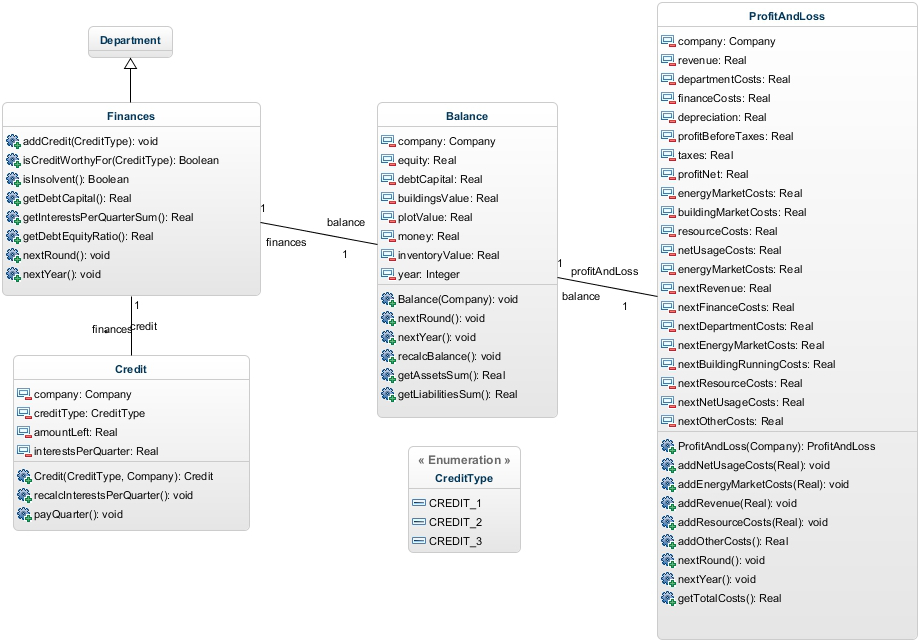
\includegraphics[width=1.0\textwidth]{se-wa-jpg/finances}
\caption{Klassendiagramm zum Bereich der Finanzen}
\label{Finanzen}
\end{figure}
Die Finanzen sollen im Wesentlichen alle finanziell relevanten Aspekte des
Unternehmens abbilden. Hierzu gibt es das Department Finances, welches die
Bilanz, die Gewinn- und Verlustrechnung sowie alle vom Unternehmen aufgenommenen
Kredite verwaltet.

Im Einzelnen werden die relevantesten Methoden und ihre Aufgabe vorgestellt:\\
\textbf{Klasse Finances}
\begin{itemize}
  \item \textbf{addCredit(CreditType creditType):void}\\
  Mit dieser Methode lassen sich beliebig viele Kredite dem Unternehmen
  hinzuf�gen, wobei jeder Kredit als neues Objekt in die ArrayList ``credits''
  der Klasse Finances aufgenommen wird und der Kassenbestand des Unternehmens um die
  Darlehensh�he erh�ht wird. 
  \item \textbf{isCreditWorthyFor(CreditType creditType):boolean}
  Diese Methode gibt zur�ck, ob der vom Spiel vorgesehene maximale
  Verschuldungsgrad bei Aufnahme eines Kredits des Typs creditType �berschritten
  w�rde. Damit kann im UI eine �berpr�fung implementiert werden, die eine zu
  hohe Verschuldung eines Spielers verhindern kann.
  \item \textbf{isInsolvent():boolean}
  Gibt diese Methode true zur�ck, hat der Spieler eine zu hohe Verschuldung
  (welche durch Verluste und damit durch eine Reduktion des Eigenkapitals
  entstehen kann) und verf�gt gleichzeitig �ber einen negativen Kassenbestand.
  Ist das der Fall, hat der Spieler das Spiel verloren.
  \item \textbf{nextRound() und nextYear()}
  werden automatisch aufgerufen und f�hren die Kreditzahlungen durch.
\end{itemize}
\textbf{Klasse Credit}
\begin{itemize}
  \item \textbf{payQuarter()}
  wird jede Runde aufgerufen und f�hrt sowohl die Tilgung als auch die
  Zinszahlung durch. Bei abgezahlten Krediten betragen beide Werte 0, der
  Einfachheit halber (und der Tatsache, dass die Anzahl Kredite stark begrenzt
  ist) werden abbezahlte Kredite jedoch nicht aus der ArrayList credits der
  Klasse Finances entfernt.
\end{itemize}
\textbf{Klasse Balance}
\begin{itemize}
  \item \textbf{recalcBalance()}
  berechnet jedes Jahr die Werte der Grundst�cke und Geb�ude (AV), des Inventars
  und der Kasse (UV), des Eigenkapitals (EK) und des Fremdkapitals (FK).
\end{itemize}
\textbf{Klasse ProfitAndLoss}
\begin{itemize}
  \item \textbf{addXYZ(double amount)}
  da nicht alle Aufwendungen und Ertr�ge zum Ende jeden Jahres berechnet werden
  k�nnen, addieren diese Methoden die entsprechenden Werte f�r die jeweiligen
  A/E und speichern sie in den Attributen \textbf{nextXYZ}.
  \item \textbf{nextYear()}
  In dieser Methode wird jedes Jahr die Gewinn- und Verlustrechnung neu
  berechnet. Dazu werden die Werte der Variablen nextXYZ in die Variablen XYZ
  �berschrieben und dann auf 0 gesetzt. Alle anderen Aufwendungen und Ertr�ge
  werden nun berechnet. Anschlie�end wird der Gewinn bestimmt, von dem eine
  Steuer in H�he von 30\% abgezogen wird, sofern ein Gewinn vorhanden ist.
  Anschlie�end wird der Kassenbestand des Unternehmens um die H�he der
  anfallenden Steuern reduziert.
\end{itemize}

\begin{figure}[H]
\centering
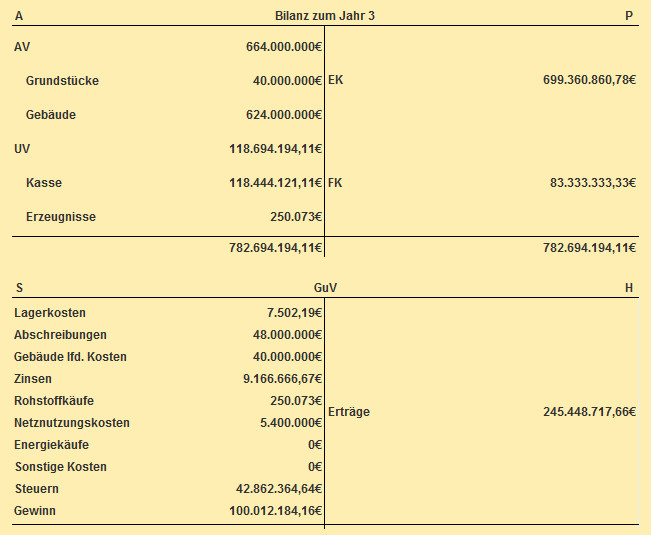
\includegraphics[width=0.8\textwidth]{se-wa-jpg/bilanz-guv}
\caption{Darstellung der Bilanz und GuV im UI}
\label{Bilanz und GuV}
\end{figure}

\section{Warenlager}

\begin{figure}[H]
\centering
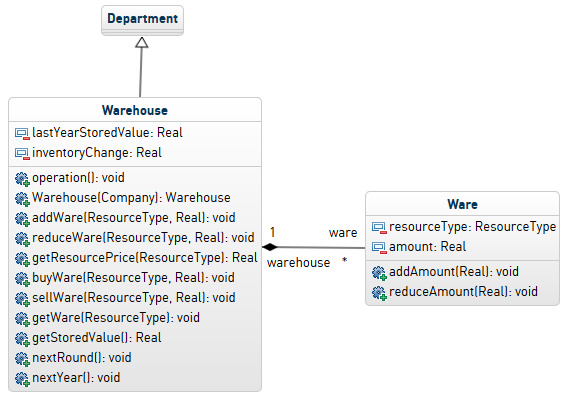
\includegraphics[width=1.0\textwidth]{se-wa-jpg/Warehouse}
\caption{Klassendiagramm zum Warenlager}
\label{Warenlager}
\end{figure}
Das Warehouse beinhaltet die Verwaltung aller Rohstoffe eines Unternehmens. Es
bildet die Lagerung durch eine Komposition mit der Klasse Ware ab, es enth�lt
Methoden zur Erh�hung und Reduzierung des Bestands sowie zum Kauf und Verkauf
von Resourcen.

\textbf{Klasse Warehouse}
\begin{itemize}
  \item \textbf{buyWare(\ldots) / sellWare(\ldots)}
  dient zum Kauf und Verkauf von Waren. Hierbei muss nicht nur der Kassenbestand
  des Unternehmens aktualisiert werden, es entstehen gleichzeitig auch
  Aufwendungen / Ertr�ge.
  \item \textbf{getStoredValue()}
  gibt den Wert der gelagerten Rohstoffe zur�ck. Dies wird zur Berechnung der
  Bilanz ben�tigt.
  \item \textbf{nextRound()}
  die Lagerkosten werden um einen von der Menge der gelagerten G�ter abh�ngigen
  Wert erh�ht.
  \item \textbf{nextYear()}
  Die Bestandsver�nderungen im Vergleich zum letzten Jahr werden berechnet. Dies
  ist f�r die Gewinn- und Verlustrechnung erforderlich, da hier Aufwendungen
  bzw. Ertr�ge entstehen.
\end{itemize}

% Wordcount: 490